\documentclass[11pt]{article}
%基于北京航空航天大学仪器科学与光电工程学院实验报告及课程报告排版得来,类似于毕业论文排版格式
%后续将更新毕业论文排版格式
\usepackage{graphicx,float}%使用图的宏包,使用图的浮动体宏包,引入参数H使图像紧跟当前文字
\usepackage{caption} %使用图表标题的宏包
\usepackage[colorlinks=true,pdfstartview=FitH,%
linkcolor=black,anchorcolor=violet,citecolor=magenta]{hyperref}%加载hyperref宏包,使用超链接
\usepackage{setspace}%用于设置行间距列间距等命令的宏包
\usepackage{array}%设置列表高度宽度的宏包
\usepackage{zhnumber}%使用中文数字编号的宏包
\usepackage{titlesec,titletoc}%使用标题自定义形式的宏包和使用目录自定义形式的宏包
\usepackage{siunitx}%物理学单位宏包
\usepackage{tabularx}%让表格宽度等于页面宽度
\usepackage{makecell}%单个表格单元调整的宏包
\usepackage{subfigure} %%使用子图的宏包
\usepackage[backend=biber,bibstyle=gb7714-1987,%nature,%%加载biblatex宏包,使用参考文献
citestyle=gb7714-1987%,backref=true%%其中后端backend使用biber
,url=false
]{biblatex}%标注(引用)样式citestyle,著录样式bibstyle都采用gb7714-2015样式
% \usepackage{pgfplots}%类似tikz的一个画图库,主要画统计图
\usepackage{../customStyle}
% \usepackage{customFont}%自行编写的字体命令库,基于CJK宏包
% \usepackage{bh_style}%自行编写的风格文件,基于使用习惯和格式要求
% \usepackage{math_formulate}%自行编写的数学公式命令库,基于amsmath宏包
% \usepackage{picture}%集成图形绘制库,主要包括了tikz和pgfplots两大主流宏包
% \usepackage[lite,subscriptcorrection,slantedGreek,nofontinfo]{mtpro2}%使用mathtimepro2商业字体作为数学环境,并不推荐

%biblatex宏包的参考文献数据源加载方式,注意book.bib应当与.tex文件在同一目录下,不然有可能会报错
\addbibresource[location=local]{book.bib}
% % \bibliographystyle{gbt7714-numerical}
%%% 下面的命令重定义页面边距,使其符合中文刊物习惯 %%%%
% \addtolength{\topmargin}{2.5cm}
\setlength{\oddsidemargin}{0.63cm}  % 3.17cm - 1 inch
\setlength{\evensidemargin}{\oddsidemargin}
% \setlength{\textwidth}{14.66cm}
% \setlength{\textheight}{24.00cm}    % 24.62

\graphicspath{{./fig}}

\begin{document}
{
\pagestyle{empty}
\begin{figure}
  
\includegraphics{title.jpg}
\end{figure}
\begin{center}

  \begin{figure}[h]

    \centering
    
\includegraphics[]{title.png}\par
    \vspace{4em}
    \large{\yihao\lishu{2023-2024学年第一学期}}
    \vspace{6em}
  \end{figure}

  \large{\erhao\lishu{微弱信号}}\par
  \large{\erhao\lishu{课程作业合集}}
  \vspace{8em}

  \begin{spacing}{2.0}
    \begin{tabular}{cc}


      {\xiaoerhao\lishu{班\quad \quad 级}} & {\heiti{\dlmu{SY23173}}}    \\
      {\xiaoerhao\lishu{学\quad \quad 号}} & {\heiti{\dlmu{SY2317301} }} \\
      {\xiaoerhao\lishu{姓\quad \quad 名}} & {\heiti{\dlmu{陈博非} }}       \\
      {\xiaoerhao\lishu{日\quad \quad 期}} & {\heiti{\dlmu{\today} } }   \\
    \end{tabular}
  \end{spacing}
\end{center}
\thispagestyle{empty}
}


\newpage
%手动分页
\pagenumbering{roman}

\setcounter{tocdepth}{3}
%设定目录深度                      
\tableofcontents
%列出目录
\newpage

\pagenumbering{arabic}
\setcounter{page}{1}
\section{第一章作业}
无
\section{第二章作业}
无
\section{第三章作业}
\subsection{第一题}
{\heiti 阿伦方差的定义、计算方法、及物理含义。}\par
阿伦方差\textit{Allan Variance}定义为,带有时变特性的信号量在一段采样时间内平均值所对应的误差方均根\textit{RME}。\par
其计算方法如下式所示:
\begin{equation}
  \sigma^2(\tau)=\frac{1}{2(N-1)}\sum_{i=1}^{N-1}(\bar{x}_{i+1}-\bar{x}_i)^2
\end{equation}\par
其中$\bar{x}_i$为采样点的平均值,$N$为采样点数,$\tau$为采样点间隔即采样周期。\par
阿伦方差的基本逻辑就是让数据序列做一阶差分后再重新计算标准方差\cite{HKJC202304012},其物理含义是:在采样时间内,信号的变化量的平均值,在工程上常用于表征信号的时域频率稳定度。\par
\subsection{第二题}
{\heiti 用阿伦方差与求统计平均及均方差在误差描述方面的差异、及优缺点。}\par
阿伦方差与统计平均的差异在于,阿伦方差是对信号的变化量进行统计,其计算过程中使用到了样本的平均值和均方差,样本的平均值多被认为是一个随机变量;而统计平均与均方差是直接对样本计算,样本值可以认为是一个确定量。一切可观测的宏观物理量都是对应的微观物理量的统计平均值,从这个意义上来说,可以认为统计平均和均方差是采样间隔极小的阿伦方差。\par
阿伦方差在分析陀螺性能上具有优越性,可以快速地确定噪声参数;但是阿伦方差只能用于求解静态的噪声特性,在实际使用中均受到动态特性的影响,动态情况下的噪声差异可达数量级别的差异。而统计平均与均方差是一切样本都具有的特性,因此可以通用。
\subsection{第三题}
{\heiti 高斯分布白噪声经过模数转换后均值、方差、相关函数的分析。}\par
先行跳过。
\section{第四章作业}
无
\section{第五章作业}
\subsection{第一题}
{\heiti 给出一个低噪声前置放大器的设计/测试/应用实例。}\par
设计实例:如亚诺德公司设计的AD797低噪声放大器,其噪声参数列表如下:\par
\begin{table}[H]
  \centering
  \renewcommand{\arraystretch}{1.5}
  \caption{AD797低噪声放大器噪声参数表}
  \begin{tabular}{c|c|c|c}
    \hline
    噪声&典型值&最大值&备注\\\hline
    输入电压噪声&$0.9 \mathrm{nV}/\sqrt{\mathrm{Hz}}$&$1.2\mathrm{nV}/\sqrt{\mathrm{Hz}}$&$1 \mathrm{kHz}$\\\hline
    输入电压噪声&$50 \mathrm{nV}$&&$0.1 \mathrm{Hz}$至$10 \mathrm{Hz}$,峰峰值\\
    \hline
  \end{tabular}
\end{table}
测试实例:?
应用实例:在无线通信领域,用于接收机接收无线信号;在精密测量领域,如扫描隧道显微镜前置放大器放大电子束成像信号;在生物医学领域,如心电图设备和脑电图设备放大生物电信号。\par
\subsection{第二题}
{\heiti 运算放大器是否适合作为低噪声前置放大器?为什么?}\par
运算放大器不适合作为低噪声前置放大器,因为普通运放内部的噪声较大,经多级运算放大输出后将产生极其显著的噪声影响。通常应当选取低噪声的放大器。
\section{第六章作业}
{\heiti 调研一个典型的光学干涉测量系统。通过对光学干涉测量的原理分析,对比论述光学干涉测量与电路的相干检测的技术特征。作业形式:报告,不少于1000 字。}
本次预计调研的光学干涉测量系统是激光干涉仪,激光干涉仪原理来源于迈克尔逊干涉仪,现在是一种较为完善的高精度测量仪器,本次调研报告的主要结构分为以下内容:\par
第一节,激光干涉仪的原理; \par
第二节,激光干涉仪主要的干扰与噪声,以及对应的补偿方案;\par
第三节,现行的激光干涉仪与电路相干检测的技术特征对比;\par
\subsection{激光干涉仪的原理}
激光干涉仪的原理与迈克尔逊干涉仪的原理相同,都是利用光的干涉原理,通过光程差的变化来测量物体的位移。激光干涉仪的光路如下图所示:
\begin{figure}[H]
  \centering
  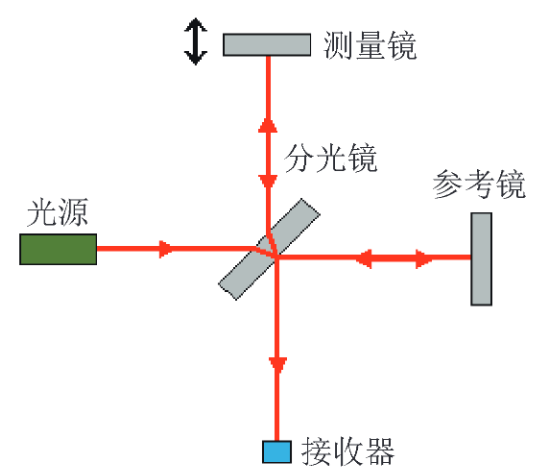
\includegraphics[width=0.8\textwidth]{激光干涉仪光学系统.png}
  \caption{激光干涉仪光学系统}
  \label{fig:激光干涉仪光学系统}
\end{figure}
激光干涉仪以稳频激光器作为光源,把被测量物体引入干涉仪的一支光路中,通过测量由于两支光路 光程差变化引起的干涉条纹变化,可以获得与几 何路程和介质折射率相关的信息,实现以激光波 长作为标尺对被测长度的测量\cite{HKJC202301007}。\par
入射的光束是同光程同相位的相干激光,经过分光镜后变为两束光,一束经过参考镜反射回接收器,其飞行光程即为光源与参考镜的距离以及参考镜虚像与接收器的距离乘以空气的折射率,记为参考光束;而另一束光经过分光镜到达测量镜,其入射到分光镜和从分光镜出射至接收器均与参考光束相同,唯有从分光镜出射至测量镜的来回光程不同,与参考光束相比,其光程将随测量镜相对零初始位置的测量位移$d$而变化$2n_0d$,其中$n_0$是空气的折射率,因此可算出对应的相位差为:
\begin{equation}
  \Delta\varphi=\frac{2\pi}{\lambda}\Delta L=\frac{4\pi n_0d}{\lambda}
  \label{eq:相位差}
\end{equation}\par
在实验中一般通过数环的吞吐数量计算相位差,从而计算出位移,每一个环吞吐一次,对应相位差改变$2\pi$,因此每吞吐一次对应位移为$\frac{\lambda}{2n_0}$,当吞吐的环数达到$N$次时,对应的位移为:
\begin{equation}
  d=\frac{\lambda}{4n_0}N
  \label{eq:位移}
\end{equation}\par
激光干涉仪采用与实验数吞吐相同的原理,不过是通过感光元件与计数器实现的,最终计数器计算得到的吞吐环数$N$,再代入式\ref{eq:位移}即可得到位移$d$。\par
\subsection{激光干涉仪的干扰与噪声}
实际使用中,往往不是如分析状态下的理想情况,而是存在各种各样的干扰与噪声,这些干扰与噪声会对激光干涉仪的测量结果产生影响,因此需要对其进行分析与补偿。下面分别对干涉仪遇到的各种噪声进行分析。\par
\subsubsection{光源噪声}
光源出射的激光具有单色性和相干性,但是仍然意味着激光的频谱带宽存在,因此出射的激光波长是以额定波长$\lambda_0$为中心的概率分布,在高精度测量中,由于频率变化带来的测量距离变化会造成相当大的影响,以氦氖激光器波长为例,其波长为$632.8\mathrm{nm}$,频率为$473.6\mathrm{THz}$,频率变化微小量$1\mathrm{GHz}\approx 2\times 10^{-6}\nu$,对应的距离变化为:
\begin{equation}
  \Delta d=\frac{c}{2\nu^2}\Delta\nu=0.63\mathrm{nm}
  \label{eq:频率变化对应的距离变化}
\end{equation}\par
每一次吞吐即导致0.63nm的误差,多次环吞吐产生的误差不容忽略,因此需要对光源的频率进行稳定。\par
解决频率不稳定的方式一般是使用稳频光源,激光器出射的频率受到激光器谐振腔长控制,使用过程中激光器谐振腔随温度上升而膨胀是导致激光频率变化的最主要因素,一般通过热控制技术和热反馈技术,限制激光器谐振腔的长度变化,从而限制激光器频率的变化。\par
\subsubsection{光路噪声}
激光干涉仪的光路经过空气,空气折射率略大于1,在一般情况下可以忽略,空气折射率的变化也会导致测量噪声的增加,因此一般使用中需要对空气折射率进行补偿。考虑空气受气压、湿度和温度的影响最为显著,一般通过以下两种方式补偿空气折射率误差:
\begin{enumerate}
  \item 使用气压计、温度计和湿度计,根据空气折射率与这三个量的经验公式折算出空气折射率,并代入当前计数器得到的吞吐数,从而算出经过补偿后的光程并由此得到距离;
  \item 分离光源与光路,光源随使用时间增加而发热量增大,因此光源附近的空气膨胀最为剧烈,使用分离式的分光镜将测量使用的两支光路与激光器隔开,避免了激光源对测量介质的影响。
\end{enumerate}
\subsection{激光干涉仪与电路相干检测对比}
国内高端激光干涉仪市场现主要以进口产品为主,雷尼绍公司占有80\%以上的市场份额,美国安捷伦公司、德国Zeiss公司、英国Renishaw公司等也有一定的市场份额。国内的激光干涉仪市场主要以雷尼绍公司为主,其产品的价格在几十万到上百万不等,科研院所,计量院绝大部分用雷尼绍。精度为0.5ppm。以雷尼绍XL-80激光干涉仪为例\cite{plc_renishaw_nodate},其技术参数主要有激光稳频精度、线性度、动态特性、测量距离、测量速度以及预热时间。与电路相干测量方式相比,光学干涉测量不需要模拟电路对信号的运算与放大,其信号的放大过程在光学干涉阶段已经完成,放大的信号(如干涉圆环)通过光学传感器予以接收,两者具有的最主要区别与联系如下表所示
\begin{table}
  \caption{光学干涉测量与电路相干检测的对比}
\begin{tabular}{|m{0.3\textwidth}<{\centering}|m{0.3\textwidth}<{\centering}|m{0.3\textwidth}<{\centering}|}
  \hline
  项目&光学干涉测量&电路相干检测\\\hline
  调制方式&光束调制&周期电信号调制\\\hline
  解调方式&光束叠加干涉,使用光学传感器接收干涉图像&电路相关检测,使用电子电路或微机完成运算\\\hline
\end{tabular}
\end{table}
除以上对比以外,光学干涉测量与电路相关检测还具有高度的类似性,如下表所示:
\begin{table}
  \caption{光学干涉测量与电路相干检测的联系}
\begin{tabular}{|m{0.3\textwidth}<{\centering}|m{0.3\textwidth}<{\centering}|m{0.3\textwidth}<{\centering}|}
  \hline
  项目&光学干涉测量&电路相干检测\\\hline
  放大过程&光束干涉将微小位移信号转换为可视的干涉图像&电子电路通过高频调制后放大解调,从互不相关的噪声量提取微弱信号\\\hline
  相关检测实现方式&激光器的稳频特性,保证不同频率的激光不产生光拍频&可变延时环节,使用积分器检测相关情况\\\hline
  相敏检测实现方式&相敏检测内生于两束光的干涉中,相位差直接决定干涉的图像形状&两路信号相乘后进行低通滤波,检测同时刻两路信号的相关函数\\\hline
\end{tabular}
\end{table}
\newpage
\printbibliography[heading=bibliography,title=参考文献]
\end{document}
